\documentclass[10pt,a4paper,oneside]{article}
\usepackage{cmap}
\usepackage[T2A]{fontenc}
\usepackage{float}
\usepackage{listings}
\usepackage{csquotes}
\usepackage[utf8]{inputenc}
\usepackage{amsmath}
\usepackage{amsfonts}
\usepackage{amssymb}
\usepackage[english, russian]{babel}%Подключаем русский язык.
\usepackage{graphicx}
\usepackage{geometry} % Меняем поля страницы.
\geometry{left=3cm} %Левое поле.
\geometry{right=2cm} %Правое поле.
\geometry{top=3cm} %Верхнее поле.
\geometry{bottom=2cm} %Нижнее поле.


%Начало документа
\begin{document}

%Создаём титульник.
\begin{titlepage}
\newpage
	%Название ВУЗа и институт.
	\begin{center}
		\Large Санкт-Петербургский Государственный Политехнический Университет\\
		Институт Компьютерных Наук и Технологий\\
	\end{center}
	%Кафедра.
	\begin{center}
		\large\textbf {Высшая школа интеллектуальных систем и суперкомпьютерных технологий}
	\end{center}
	
	%Пропуск места. 
	\vspace{5em}
	%!!!!!!!!!!!!!!!!!!!!!!!!!!!!!!!!!Название работы.
	\begin{center}
		\large{Отчёт по лабораторной работе №1 \\ на тему \\
		\textbf{Звуки и Сигналы} }
	\end{center}
	
	%Делаем пропуск и пишем студента и преподавателя.
	\vspace{25em}
	\begin{flushright}
		\textbf{Работу выполнил\\}Студент группы 3530901/80203 \\ Тарасенко Н.С.\\
		\textbf{Преподаватель\\}Богач Н.В. 
	\end{flushright}
	
	\vspace{\fill}%В самом низу
	\begin{center}
	Санкт-Петербург, 2021 год	
	\end{center}
\end{titlepage} %Закончили титульный лист.

\section{Настройка проекта}
Устанавливаем jupiter с помощью дистрибутива anaconda. Делаем fork репозитория thinkdsp и открываем необходимые файлы для работы, также создаем собственный файл, где будем работать со звуками.

\section{Скачивание звука и работа с ним}
В этом упражнении мы пользуемся помощью беслпатного ресурса с различными звуками и качаем в папку репозитория звук, подходящий для нашей лабораторной работы. В папке code файл "hard.wav" - это и есть наш звук.  Дальше мы обращаемся напрямую к файлу звука и обрезаем интервал в полсекунды
\begin{figure}[H]
        \centering
        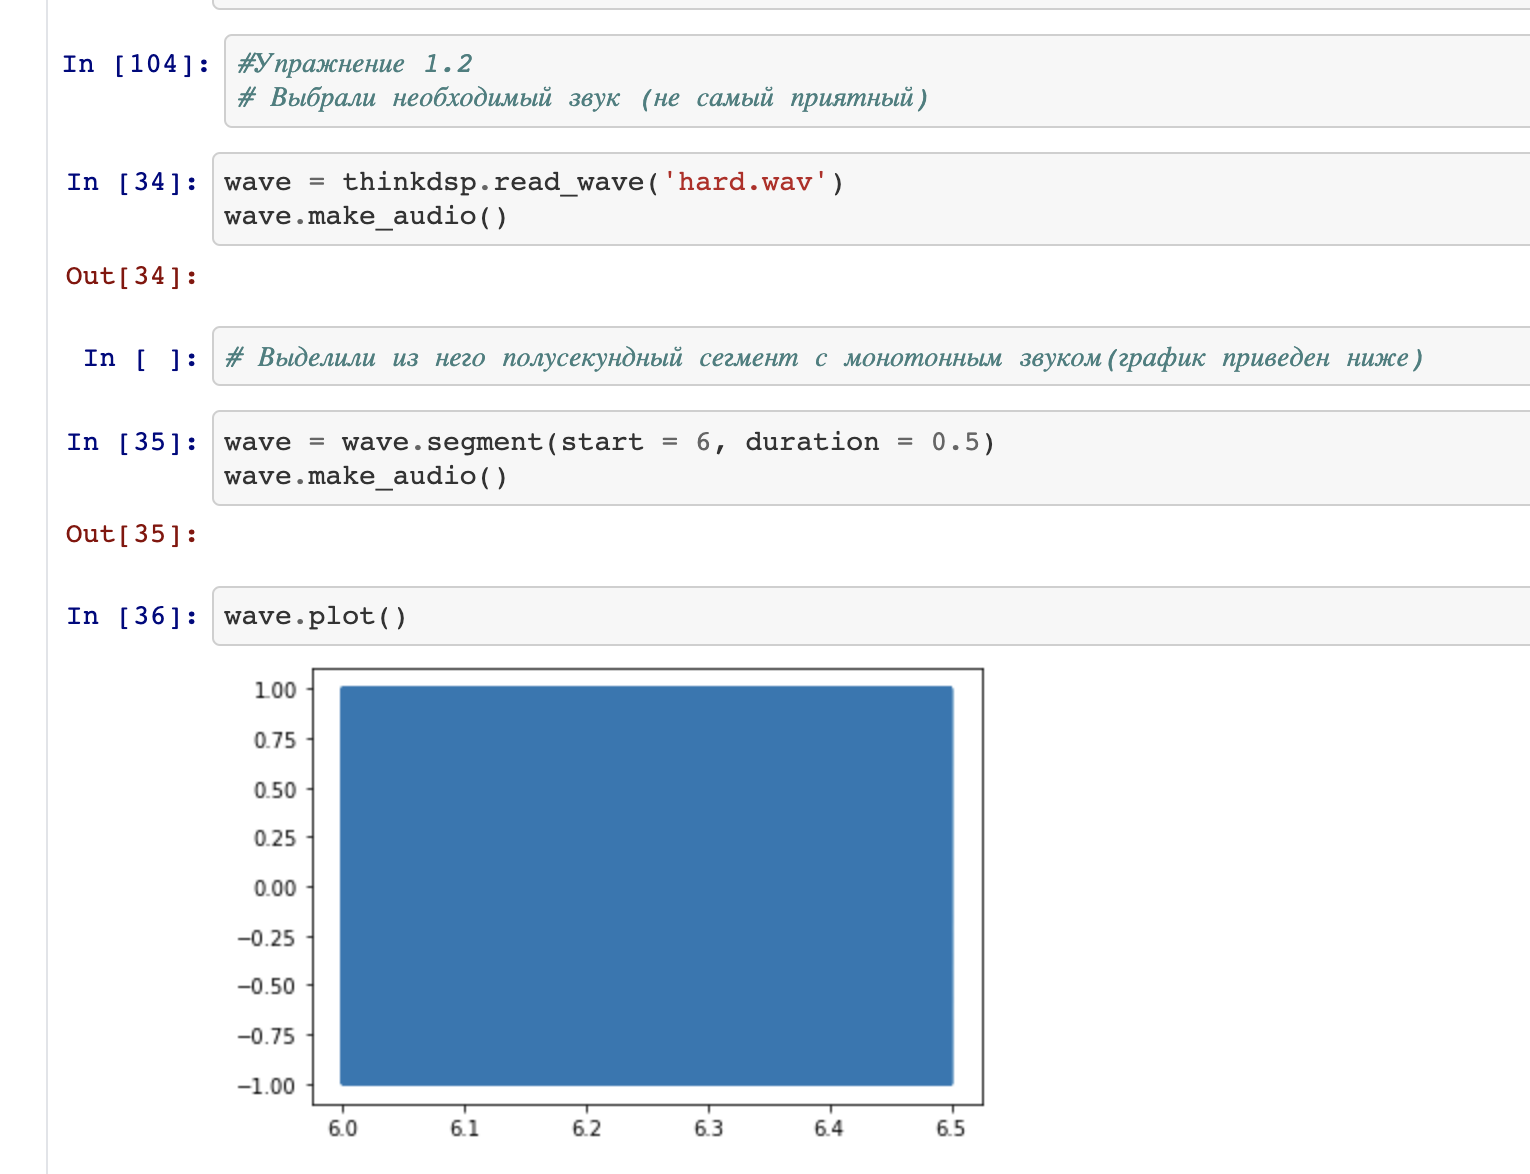
\includegraphics[width=0.75\textwidth]{Pictures/first.png}
        \caption{2}
        \label{fig:first}
\end{figure}

\section{Спектр звука}

Теперь рассмотрим спектр нашего полусекундного сегмента звука.
\begin{figure}[H]
        \centering
        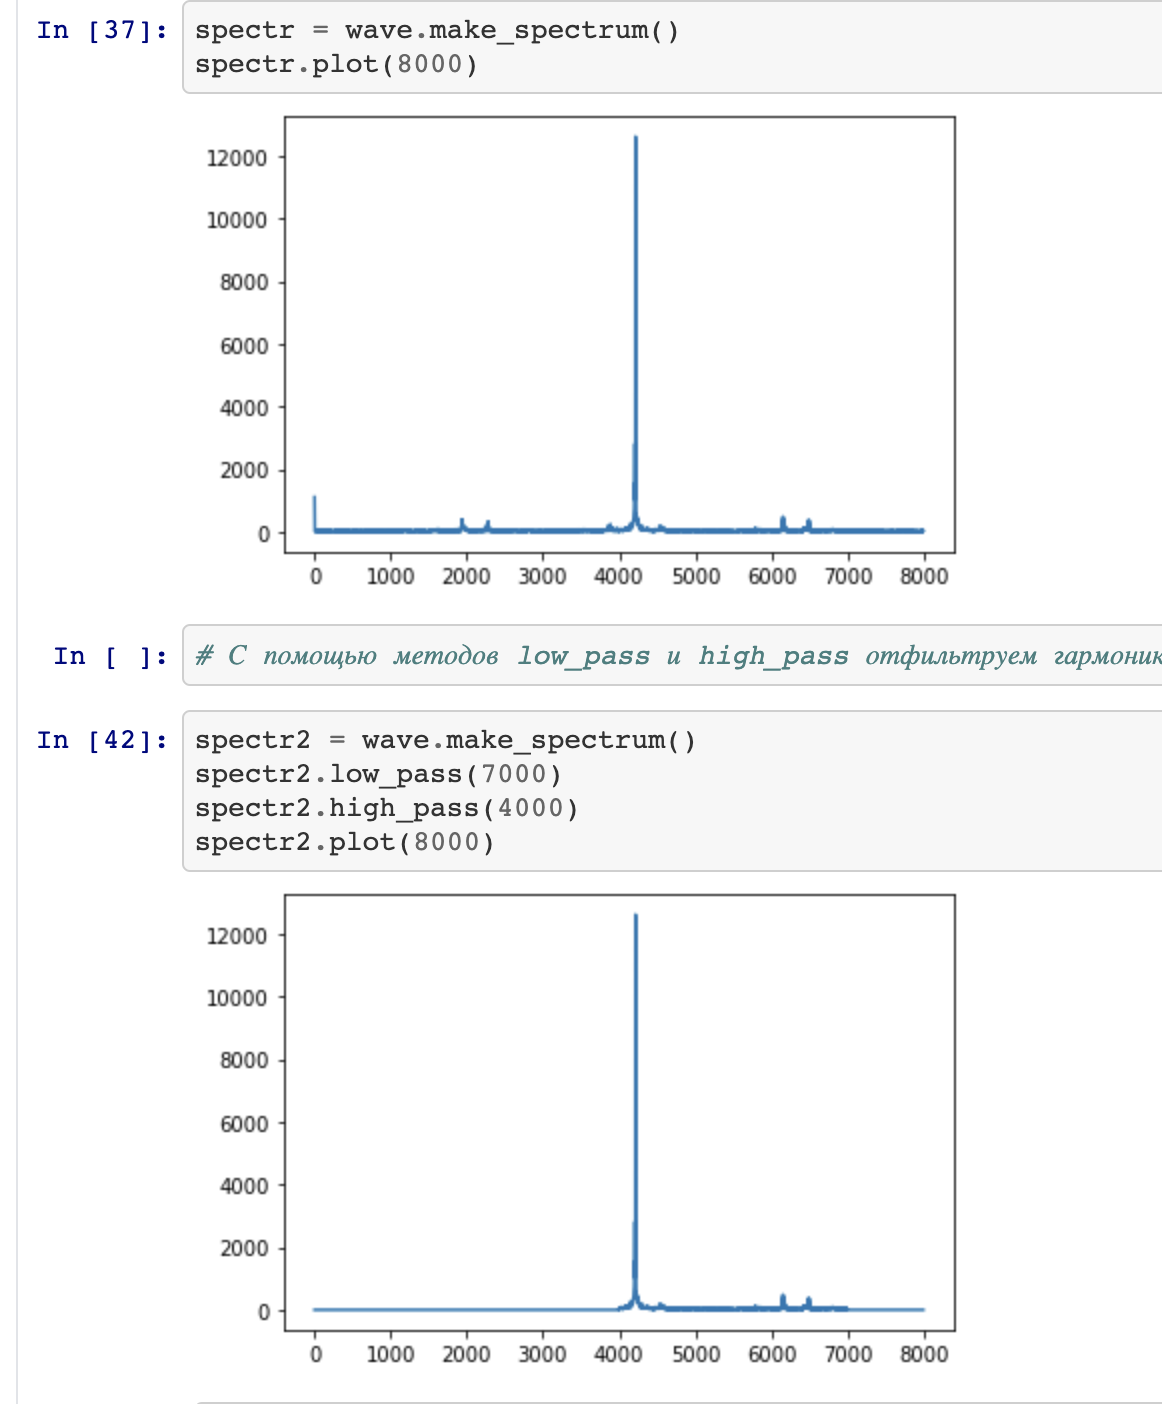
\includegraphics[width=0.75\textwidth]{Pictures/second.png}
        \caption{3}
        \label{fig:second}
\end{figure}

С помощью функций lowPass and highPass мы отфильтровали наш спектр и убрали ненужные гармоники. 

Преобразуем спектр обратно в сигнал и послушаем результат 
Звук стал более приятным и не таким ушираздирающим, стал тише и похожим уже не скример, 
а на аппарат сердцебиения (когда сердце уже не бьется )
\begin{figure}[H]
        \centering
        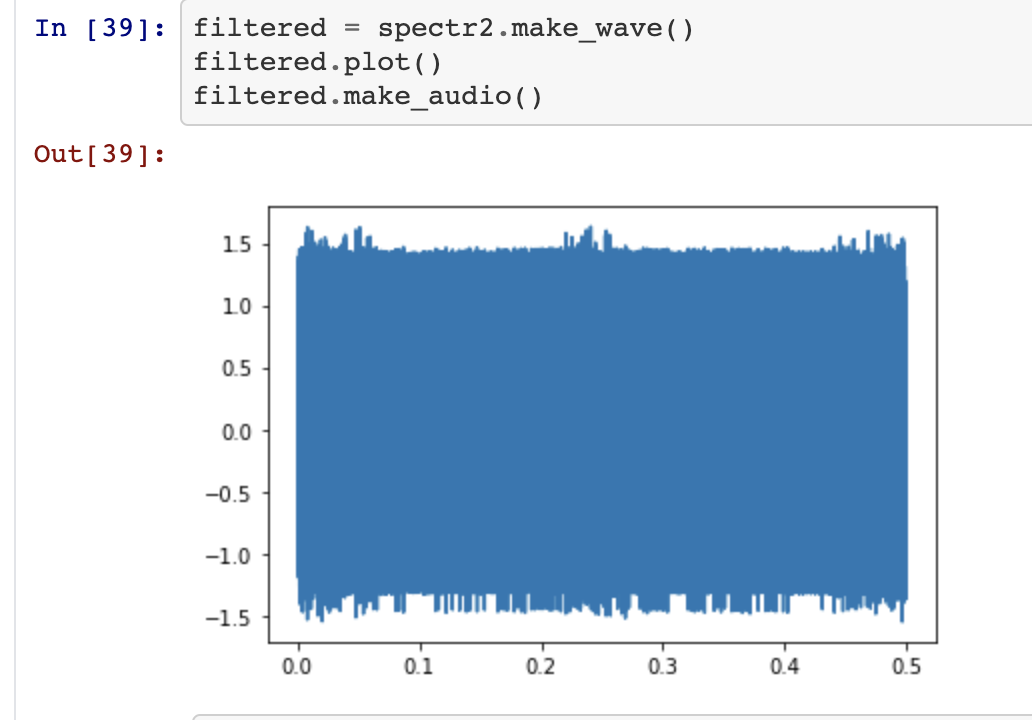
\includegraphics[width=0.75\textwidth]{Pictures/fourth.png}
        \caption{4}
        \label{fig:fourth}
\end{figure}
\section{Создание сложного сигнала}

Создадим сложный сигнал

\begin{figure}[H]
        \centering
        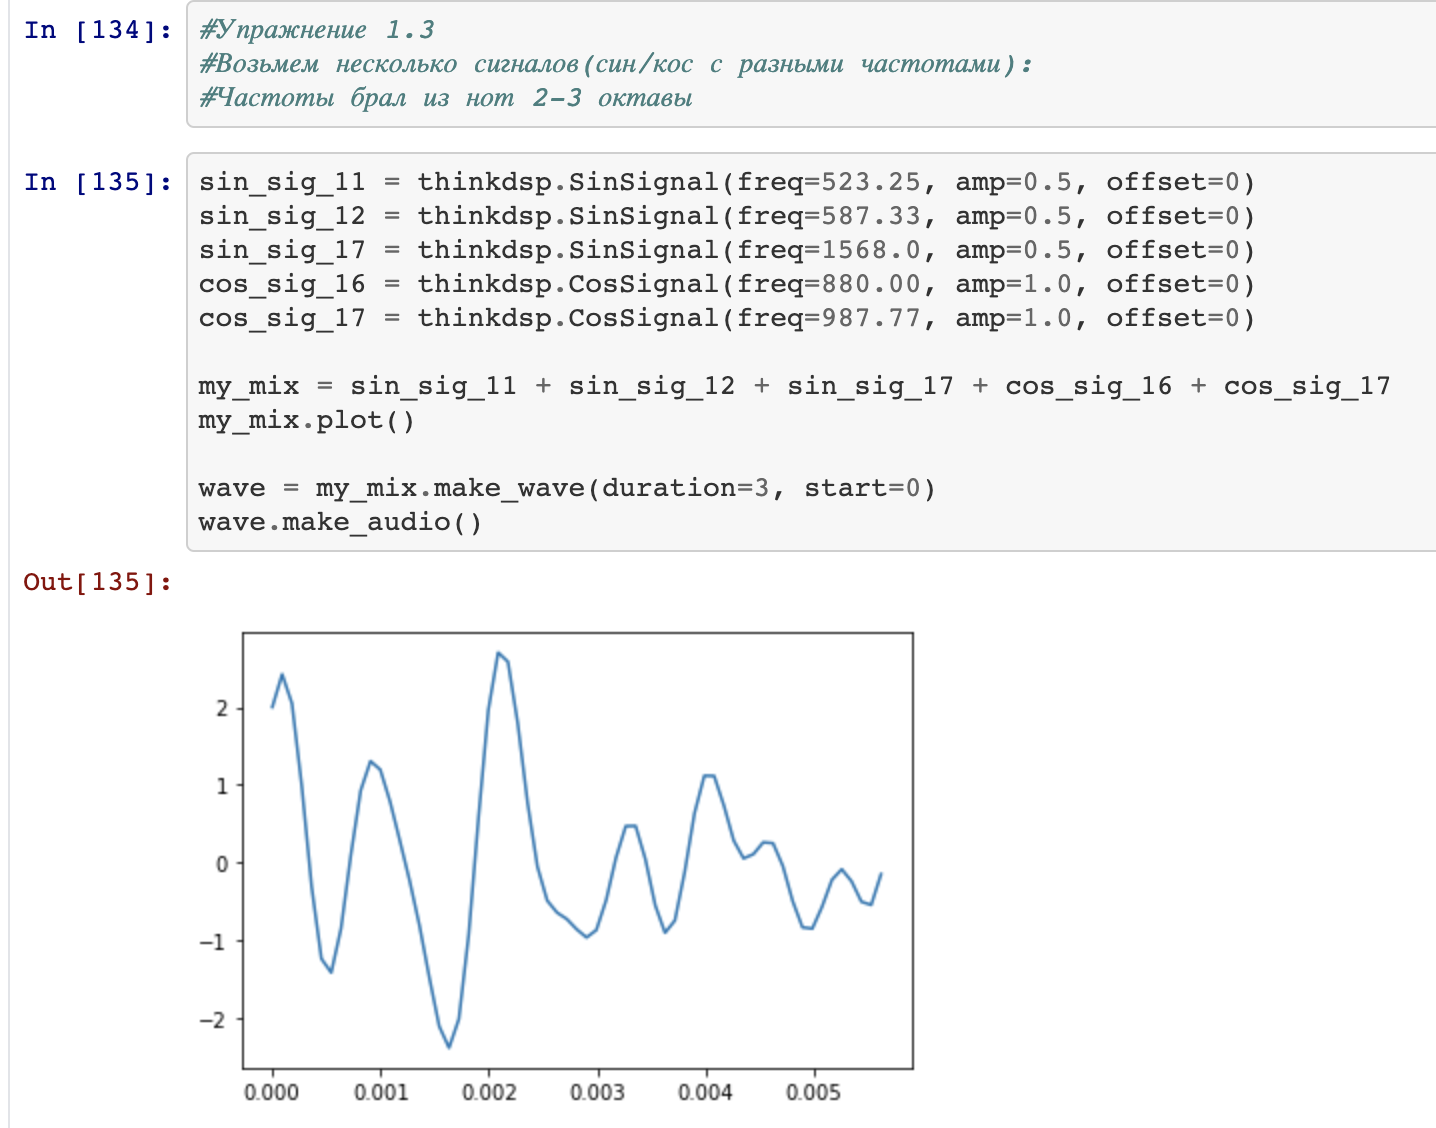
\includegraphics[width=0.75\textwidth]{Pictures/third.png}
        \caption{3}
        \label{fig:third}
\end{figure}

Наш сигнал получился схожим с сигналом автомобиля.

Сейчас выведем спектр нашего сигнала. И посмотрим на результаты.
\begin{figure}[H]
        \centering
        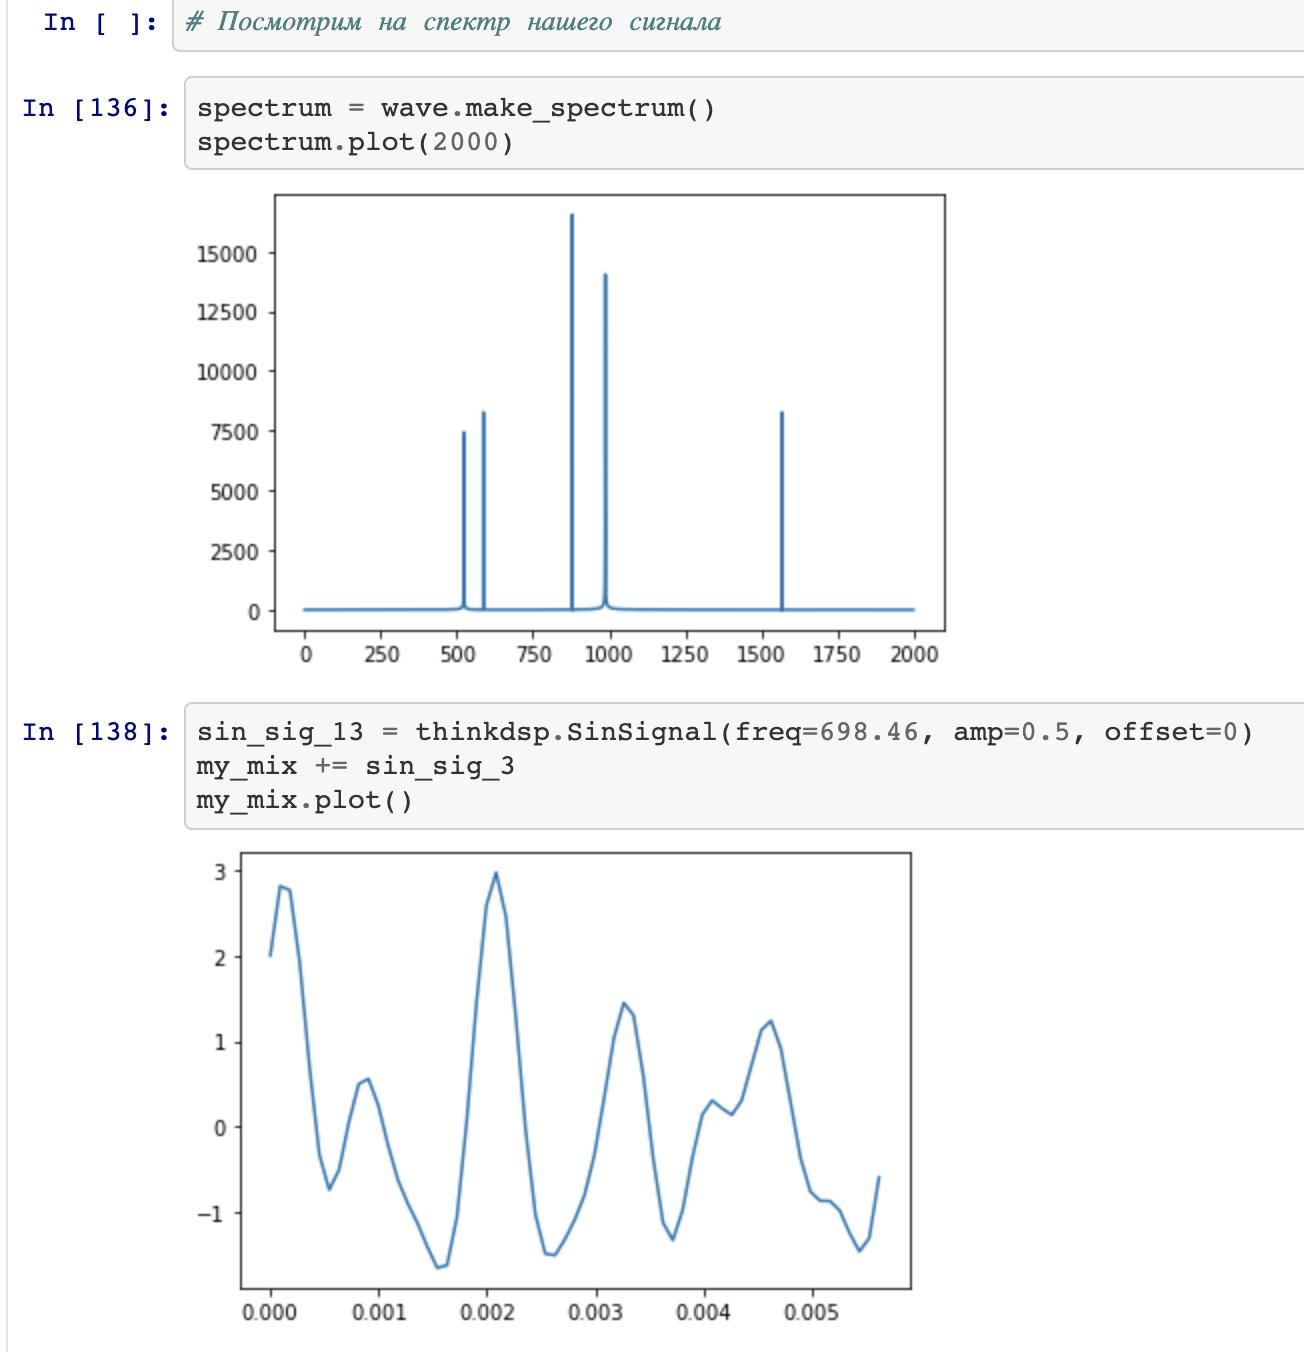
\includegraphics[width=0.75\textwidth]{Pictures/fifth.png}
        \caption{Исходный звук}
        \label{5}
\end{figure}

\begin{figure}[H]
        \centering
        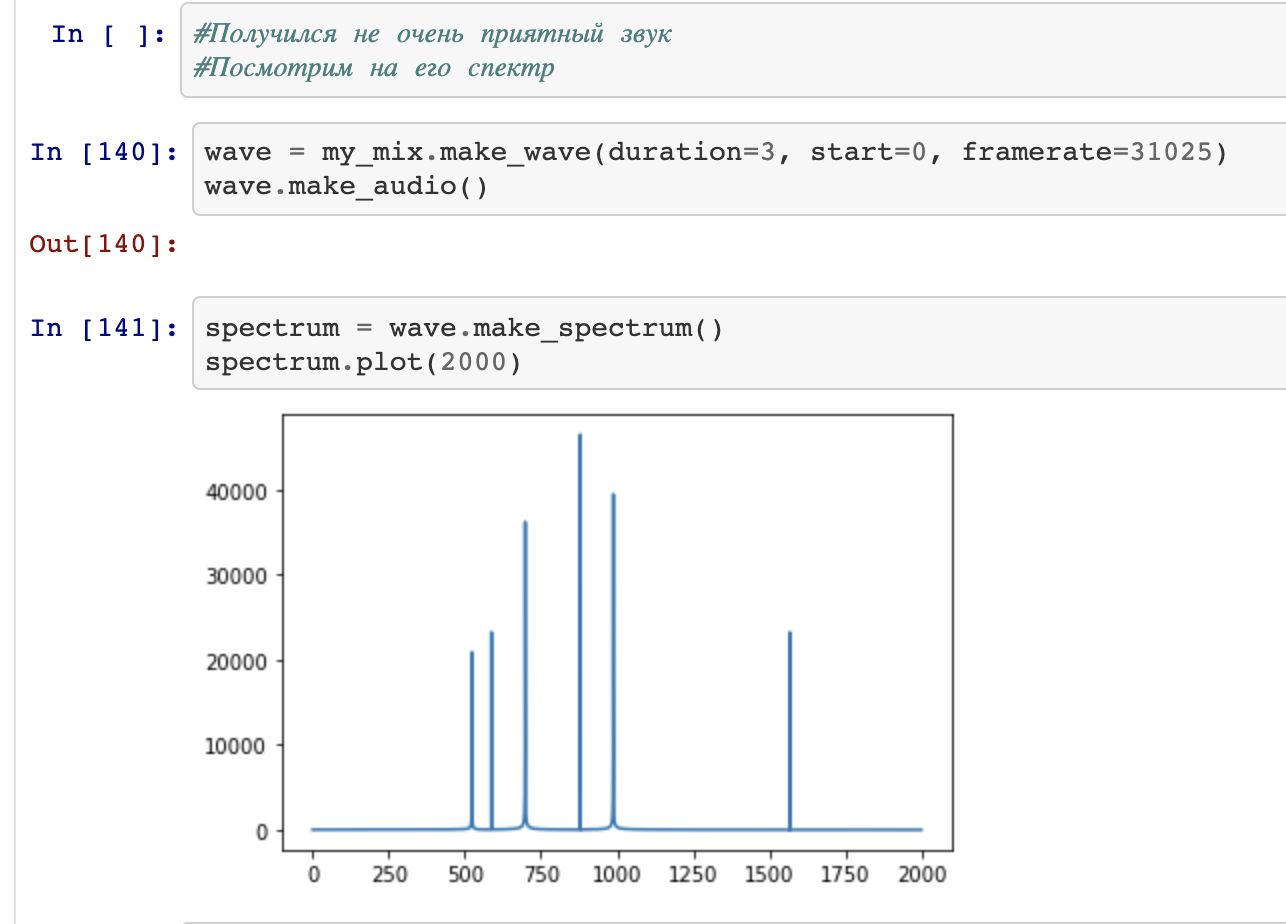
\includegraphics[width=0.75\textwidth]{Pictures/sixth.png}
        \caption{6}
        \label{fig:sixth}
\end{figure}

\section{Функция изменения длины сигнала}
Мы написали метод а дальше создали 2 сигнала и применили разные коэффициенты.
Первый маленький коэф делает сигнал короче, а больший коэффициент увеличивает длинну сигнала.
\begin{figure}[H]
        \centering
        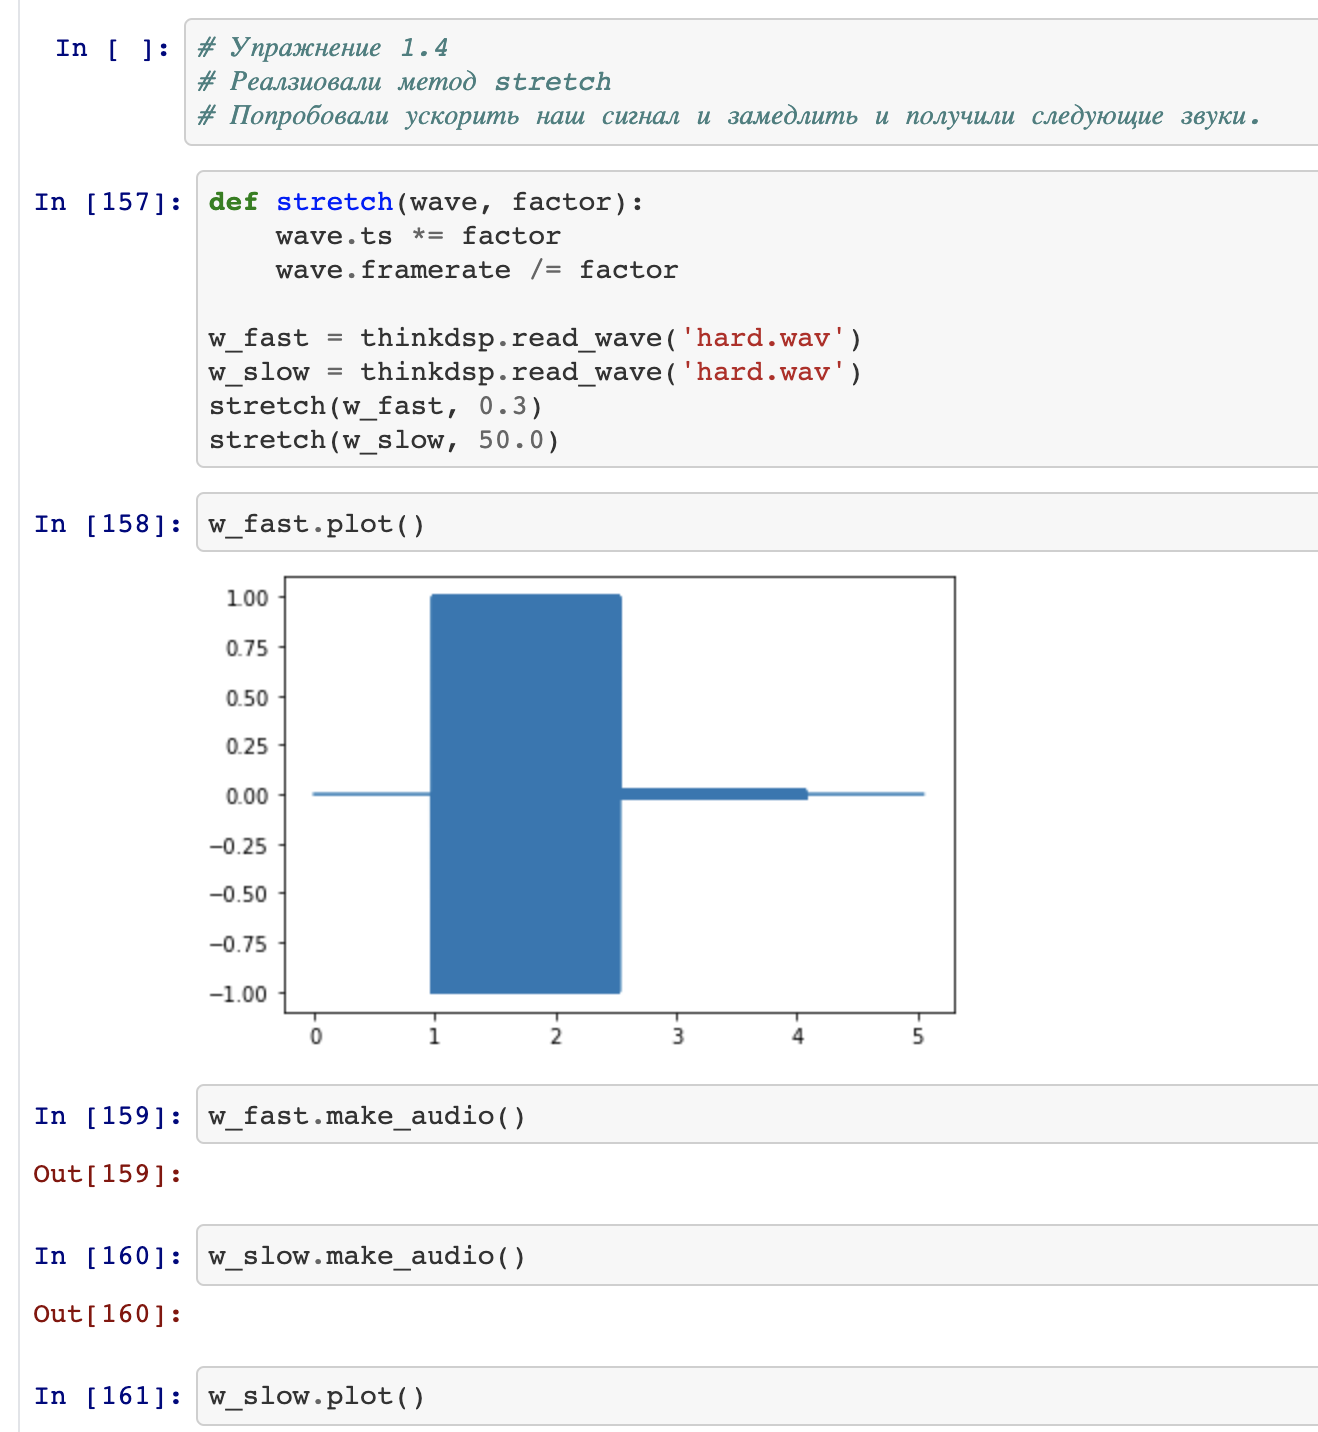
\includegraphics[width=0.75\textwidth]{Pictures/seventh.png}
        \caption{7}
        \label{fig:seveth}
\end{figure}

\begin{figure}[H]
        \centering
        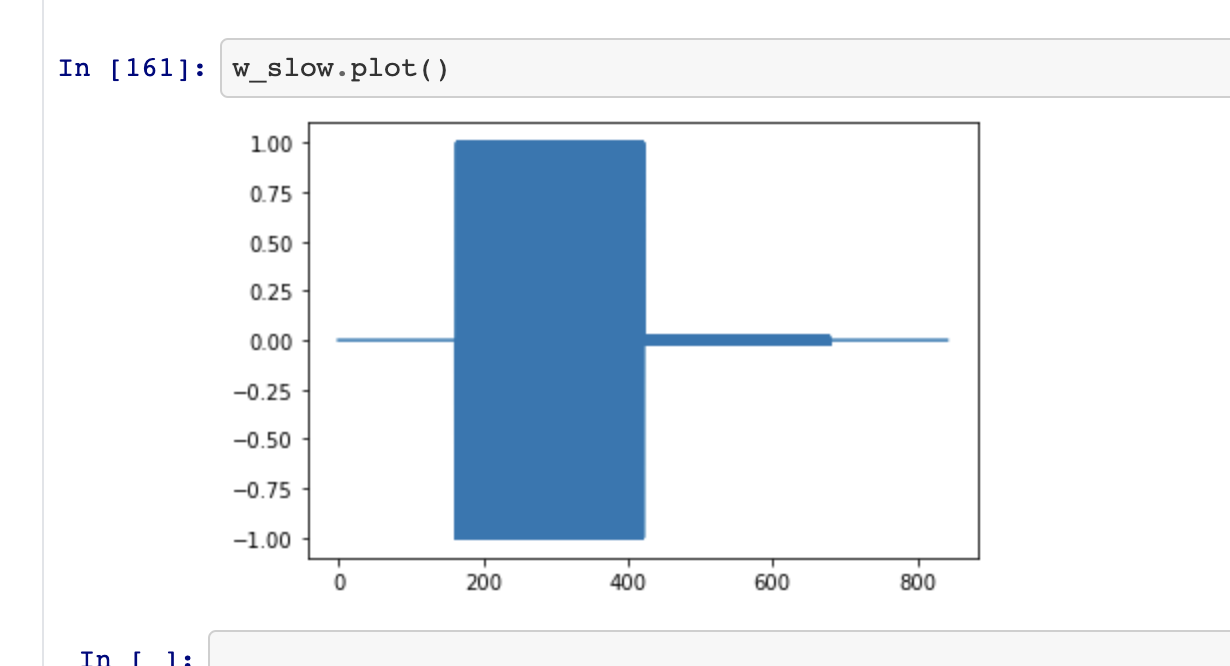
\includegraphics[width=0.75\textwidth]{Pictures/eighth.png}
        \caption{8}
        \label{fig:eight}
\end{figure}
Во время выполнения лабораторной работы получены навыки работаты со звуками, волнами и спектрами. Также я научился находить более высокие и фундаментальные пики, определять частоту, а также ускорять и замедлять звуки и строить графики.
\end{document}